\documentclass[20pt, a1paper, landscape, margin=0mm, innermargin=12mm, blockverticalspace=7mm, colspace=14mm, subcolspace=8mm]{tikzposter}

\usepackage[utf8]{inputenc}
\usepackage[T1]{fontenc}
\usepackage{booktabs}
\usepackage{enumitem}
\setlist[itemize]{nosep, itemsep=2mm, leftmargin=1.4em, topsep=1mm}
\usepackage{amsmath}
\usepackage{graphicx}

% Kill the "LaTeX TikZposter" watermark
\tikzposterlatexaffectionproofoff

% ── colour scheme: slate navy + burnt orange accent ──
\definecolor{posterink}{RGB}{28,36,54}       % near-black navy
\definecolor{posternavy}{RGB}{38,64,102}     % header / block titles
\definecolor{posteraccent}{RGB}{178,74,43}   % burnt orange
\definecolor{posterbg}{RGB}{236,233,226}     % warm grey canvas (cards pop)
\definecolor{posterblock}{RGB}{255,255,255}  % block background
\definecolor{postertint}{RGB}{225,232,241}   % light navy tint (take-home)
\definecolor{postergood}{RGB}{47,109,79}     % green for "fixed"
\definecolor{posterbad}{RGB}{161,58,46}      % red for "broken"

\definecolorstyle{AuditStyle}{}{
  \colorlet{backgroundcolor}{posterbg}
  \colorlet{framecolor}{posternavy}
  \colorlet{titlefgcolor}{white}
  \colorlet{titlebgcolor}{posternavy}
  \colorlet{blocktitlebgcolor}{posterblock}
  \colorlet{blocktitlefgcolor}{posternavy}
  \colorlet{blockbodybgcolor}{posterblock}
  \colorlet{blockbodyfgcolor}{posterink}
  \colorlet{innerblocktitlebgcolor}{posterblock}
  \colorlet{innerblocktitlefgcolor}{posterink}
  \colorlet{innerblockbodybgcolor}{posterblock}
  \colorlet{innerblockbodyfgcolor}{posterink}
  \colorlet{notefgcolor}{posterink}
  \colorlet{notebgcolor}{posterblock}
}

\usetheme{Default}
\usecolorstyle{AuditStyle}
\useblockstyle{Minimal}
\usetitlestyle{Filled}

\settitle{\centering
  {\Huge\bfseries\textcolor{white}{Are broker probabilities trustworthy?}}\\[4mm]
  {\LARGE\textcolor{white}{A calibration audit of three production transient
    classifiers: ALeRCE, Fink \& NEEDLE}}\\[5mm]
  {\Large\textcolor{white}{Pallavi Sati \hspace{5mm}---\hspace{5mm}
    School of Physics, University of Bristol \hspace{5mm}---\hspace{5mm}
    \texttt{github.com/pallavi-2000/transient-calibration-audit}}}
}

\begin{document}

\maketitle[width=\textwidth, roundedcorners=0, linewidth=0pt, innersep=6mm,
           titletotopverticalspace=0mm, titletoblockverticalspace=7mm]

\begin{columns}

% ═══════════════════════ COLUMN 1 — problem, method, data ═══════════════════════
\column{0.28}

\block{The decision problem}{
{\bfseries LSST: $\sim$$10^7$ alerts per night. Global spectroscopy:
$\sim$$10^5$ per year.} Brokers bridge the gap with class probabilities,
which astronomers read as confidence. \textbf{That assumption has not
been systematically tested against independent spectroscopic ground
truth for production broker outputs.}

\vspace{4mm}
\centering
{\Large\bfseries The calibration test:}\\[2mm]
{\Large If the broker says $P = 0.9$,\\ is it right \textbf{90\% of the
time}?}

\vspace{4mm}
\raggedright
\begin{itemize}
  \item \textcolor{posterbad}{\textbf{Overconfident}} $\rightarrow$ silent
    failures nobody questions.
  \item \textcolor{posteraccent}{\textbf{Underconfident}} $\rightarrow$
    spectra wasted on events already classified right.
\end{itemize}
}

\block{Method}{
\centering
\textbf{BTS spectra} $\rightarrow$ \textbf{broker $P$}
$\rightarrow$ \textbf{reliability diagram} $\rightarrow$
\textbf{ECE $\pm$ CI} $\rightarrow$ \textbf{temperature scaling}

\vspace{3mm}
\begin{equation*}
\mathrm{ECE} = \sum_{m=1}^{10} \tfrac{|B_m|}{n}\,
  \bigl|\,\mathrm{acc}(B_m) - \mathrm{conf}(B_m)\,\bigr|
\end{equation*}

\raggedright
2,000-resample bootstrap 95\% CIs throughout. $T$ fitted by
\textbf{held-out CV} (grouped by object) — never on the evaluation
data. ECE is paired with \textbf{ROC-AUC}: an uninformative score can
still look calibrated.
}

\block{Data \& key numbers}{
Spectroscopic labels from the \textbf{ZTF Bright Transient Survey}
($m<18.5$) — ground truth never comes from the brokers being audited.
757 SNIa $\cdot$ 560 SNII $\cdot$ 204 SNIbc $\cdot$ 55 SLSN $\cdot$
30 TDE. Bright, low-$z$ $\Rightarrow$ an \textbf{upper bound} on brokers.

\vspace{3mm}
\centering
\begin{tabular}{lrr}
\toprule
Classifier & raw ECE & best held-out ECE \\
\midrule
ALeRCE LC ($n$=1576) & 0.259 & \textcolor{postergood}{\textbf{0.015}} \\
Fink RF ($n$=1368)   & \textcolor{posterbad}{0.464} & 0.353$^{\ddagger}$ \\
Fink SNN ($n$=1368)  & \textcolor{posterbad}{0.304} & 0.229$^{\ddagger}$ \\
NEEDLE-TH ($n$=429)  & 0.050 & class-specific \\
\bottomrule
\end{tabular}\\[2mm]
\raggedright
{\footnotesize $^{\ddagger}$best \emph{informative} correction;
isotonic gets ECE${\approx}$0.01 only by collapsing to the base rate.}
}

% ═══════════════════════ COLUMN 2 — ALeRCE ═══════════════════════
\column{0.39}

\block{ALeRCE: underconfident --- one scalar fixes the aggregate}{
\begin{center}
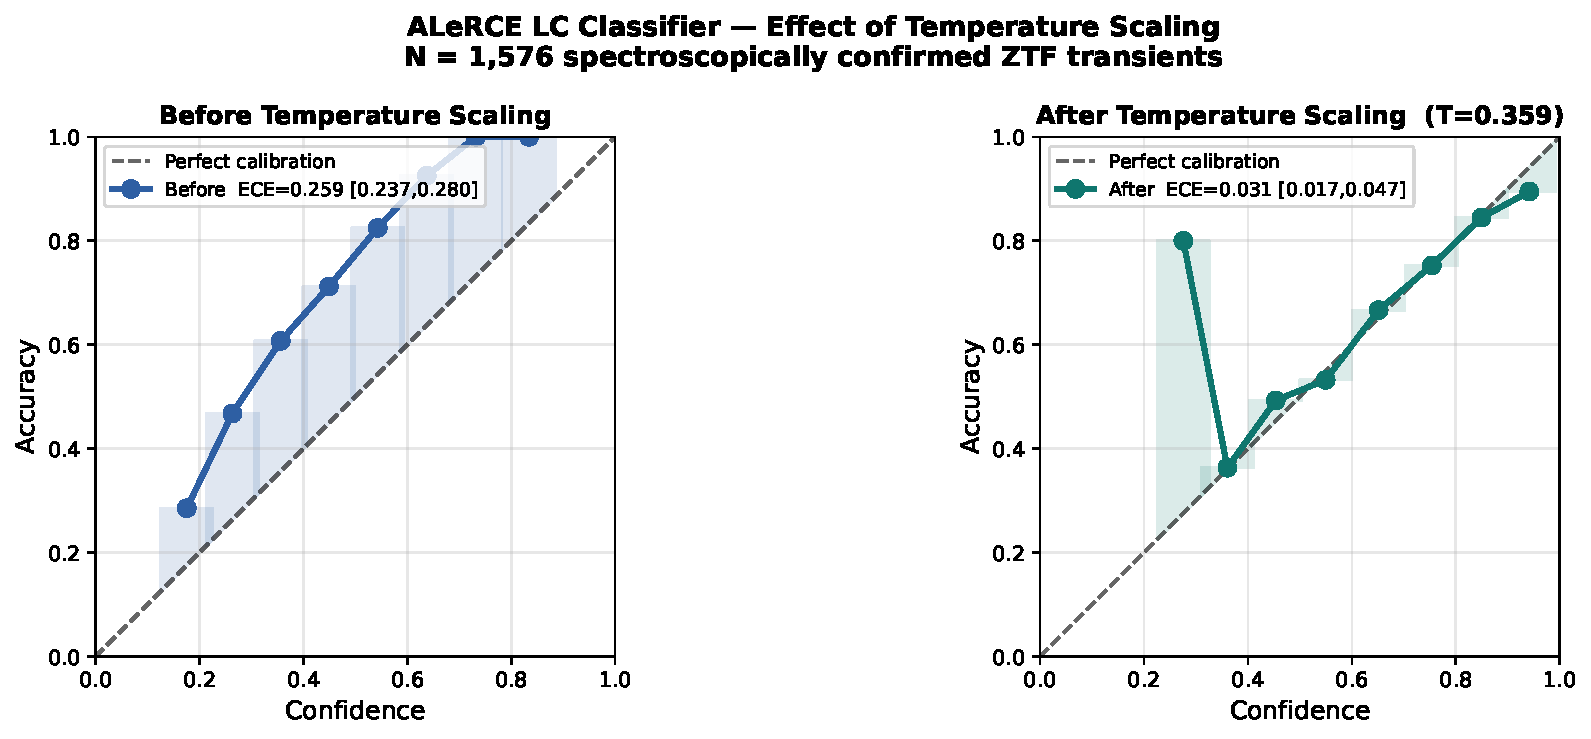
\includegraphics[width=0.92\linewidth]{../../results/figures/fig4_temperature_scaling.pdf}
\end{center}

\vspace{2mm}
Every bin sits \textbf{above} the diagonal: accuracy 0.71 vs.\ mean
confidence 0.45; $\mathrm{ECE}=0.259~[0.237, 0.280]$. One temperature
sharpens it. \textbf{Shown above: same-set fit, $0.259 \to 0.031$
(oracle upper bound). Held out: $\mathbf{0.015}$ pooled over grouped
5-fold CV ($T = 0.361 \pm 0.011$) and $\mathbf{0.024}$ on an
independent 60/40 split} — the correction generalises, with no
retraining. It is not class-uniform: SNII worsens under global $T$
($0.10 \to 0.19$), so class-aware calibration is the remaining step.

\vspace{4mm}
\begin{minipage}[t]{0.46\linewidth}
\centering
\textbf{Confidence deficit by true class}\\[2mm]
\begin{tabular}{lrrr}
\toprule
Class & $N$ & Acc & ECE \\
\midrule
SNIa  & 757 & 0.83 & \textcolor{posterbad}{0.377} \\
SNIbc & 204 & 0.83 & \textcolor{posterbad}{0.362} \\
SLSN  &  55 & 0.78 & 0.245$^{*}$ \\
SNII  & 560 & 0.49 & \textcolor{postergood}{0.103} \\
TDE   &  30 & \textcolor{posterbad}{0.00} & — \\
\bottomrule
\end{tabular}\\[2mm]
{\small $^{*}$wide CI $[0.18, 0.32]$: suggestive only}
\end{minipage}%
\hfill
\begin{minipage}[t]{0.50\linewidth}
\textbf{Why? Directly observed compression:} no object in 1,576 gets
confidence $>0.88$; among \emph{correctly classified} SNIa the max is
$0.72$ vs.\ $0.83$ accuracy. The RF's vote-averaged output range cannot
reach the accuracy of its best classes — deficit guaranteed.

\vspace{3mm}
\textbf{TDE accuracy $=$ 0.000} is not miscalibration: a headline LSST
science case \emph{absent from this classifier's output taxonomy}.
\end{minipage}
}

\block{Robustness: the result is not an artefact}{
\begin{itemize}
  \item \textbf{Classifier versions.} The sample unknowingly spanned two
    production models. Re-queried version tags (1,601/1,606):
    \texttt{hierarchical\_rf\_1.1.0} ($n{=}1346$, ECE 0.258) vs.\
    \texttt{lc\_classifier\_1.1.13} ($n{=}225$, ECE 0.260); $T$ = 0.38
    vs.\ 0.33, same sharpening regime. Pooling distorts nothing.
  \item \textbf{Binning.} Equal-mass (adaptive) bins move every headline
    ECE by $\leq 1.0\%$ — no bin-construction artefact.
  \item \textbf{Probability dilution} across 15 output classes explains
    only 3\% of the miscalibration (renormalised ECE 0.251).
\end{itemize}
}

% ═══════════════════════ COLUMN 3 — Fink, NEEDLE, takeaways ═══════════════════════
\column{0.33}

\block{Fink: no ranking signal to rescale}{
\begin{center}
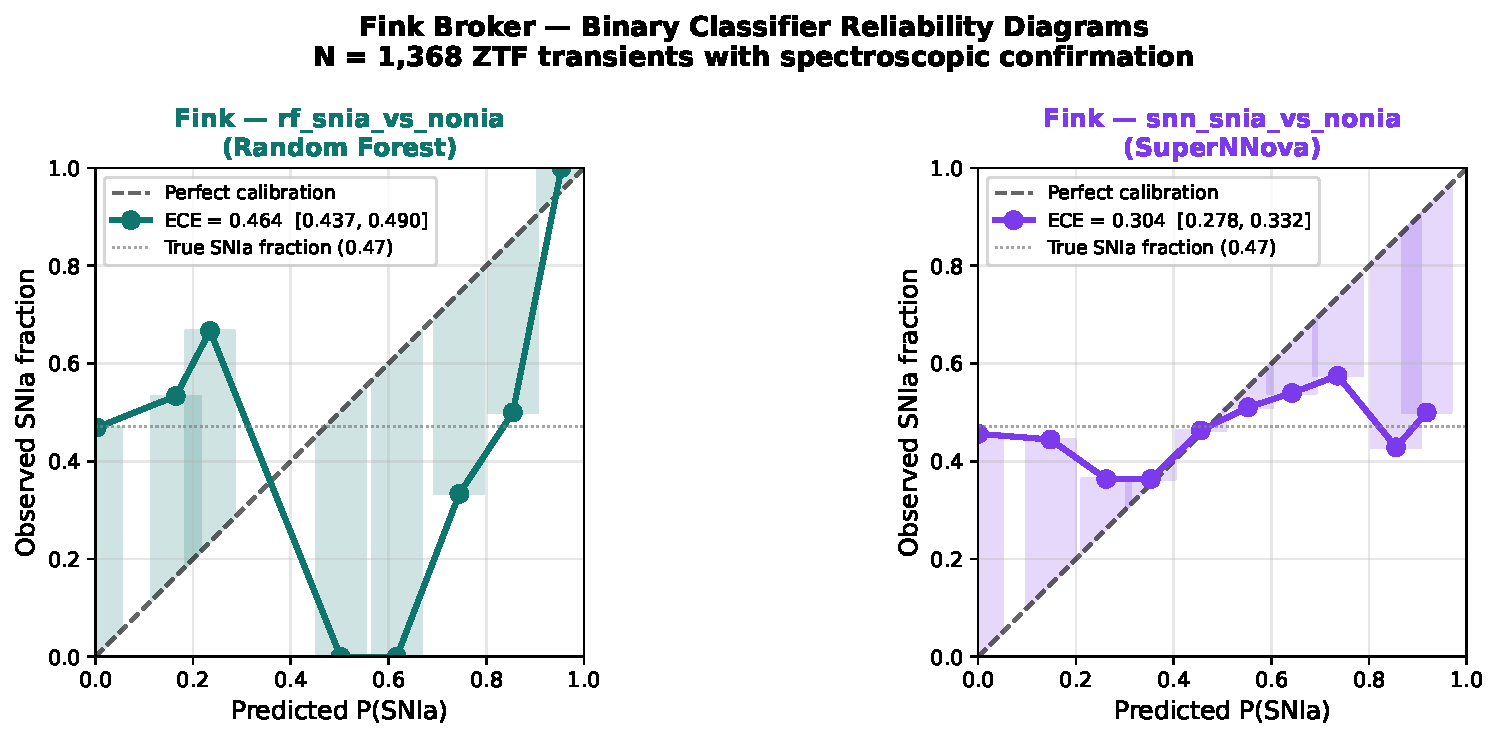
\includegraphics[width=0.54\linewidth]{../../results/figures/fig3_fink_reliability.pdf}
\end{center}

\vspace{2mm}
\centering
\begin{tabular}{lccc}
\toprule
 & ECE & post-$T$ & ROC-AUC \\
\midrule
RF  & \textcolor{posterbad}{0.464} & 0.353 & \textcolor{posterbad}{\textbf{0.502}} \\
SNN & \textcolor{posterbad}{0.304} & 0.229 & \textcolor{posterbad}{\textbf{0.525}} \\
\bottomrule
\end{tabular}

\vspace{3mm}
\raggedright
\textbf{AUC $\approx$ 0.5 = no ranking signal on this sample.}
Monotone recalibration preserves ranking, so \emph{no} post-hoc
method — temperature, Platt, isotonic, beta — can make these
informative posteriors. Early-phase proxy subsets
(\texttt{ndethist} $\leq 3$: AUC 0.500) don't rescue the RF's
documented rising-SNIa regime.
}

\block{NEEDLE: right on average, wrong per class}{
\textbf{NEEDLE-TH} — 5-CNN light-curve $+$ host-image classifier
(Sheng et al.\ 2024); \textbf{429 predictions / 278 unique
objects}. Aggregate $\mathrm{ECE}=0.050$ — but a global $T$ makes
it \emph{worse} ($\rightarrow 0.128$): the errors are
\textbf{class-asymmetric}.

\vspace{3mm}
\centering
\begin{tabular}{lcl}
\toprule
Class & $T_k$ & direction \\
\midrule
SN     & $1.58 \pm 0.10$ & overconfident \\
SLSN-I & $\mathbf{1.88 \pm 0.29}$ & \textcolor{posterbad}{severely over} \\
TDE    & $\mathbf{0.42 \pm 0.04}$ & \textcolor{posteraccent}{underconfident} \\
\bottomrule
\end{tabular}

}

{
\colorlet{blockbodybgcolor}{postertint}
\block{Take-home}{
\begin{minipage}[c]{0.75\linewidth}
\begin{itemize}
  \item \textbf{Raw broker probabilities are not calibrated}
    (ECE $0.05$--$0.46$).
  \item \textbf{One scalar fixes ALeRCE's aggregate}
    ($T{=}0.36$, $-$94\% ECE, no retraining).
  \item \textbf{Scalar rescaling fails for Fink}; NEEDLE needs
    class-specific $T_k$.
  \item \textbf{Report ECE + AUC alongside accuracy}; check
    taxonomy coverage.
\end{itemize}
\end{minipage}%
\hfill
\begin{minipage}[c]{0.21\linewidth}
\centering

\includegraphics[width=\linewidth]{repo_qr.png}\\[1mm]
{\footnotesize code $\cdot$ data $\cdot$ paper}
\end{minipage}
}
}

\end{columns}

\end{document}
